\documentclass{beamer}
\usepackage{caption}
% \usepackage{subcaption}
\usepackage{slashed}
\usetheme{Luebeck}
\setlength{\parskip}{2.5mm}
\title[Beamline for Schools\hspace{2em}\insertframenumber/
\inserttotalframenumber]{Beamline for Schools project update}
%\title[SUSY - Top background estimation]{Dilepton estimation from semi-leptonic tt-bar control}
%\author{\emph{Tim Brooks}, Glen Cowan, Aftab Alam}
\author{\emph{Tim Brooks}}
\institute{CERN / RHUL}
\date{13/3/15}
\begin{document}

\begin{frame}
\titlepage
\end{frame}

\section{BL4S}
\begin{frame}
Beamline for Schools is a competition for high-school students (16+). This is the second year of running. 212 teams have registered and will submit experiment proposals at the end of this month.

They will have access to the T9 beamline in the PS East Area.

A range of detectors will be available for them to use in their experiment.
\end{frame}

\begin{frame}{Beamline}
  \begin{figure}
    \centering
    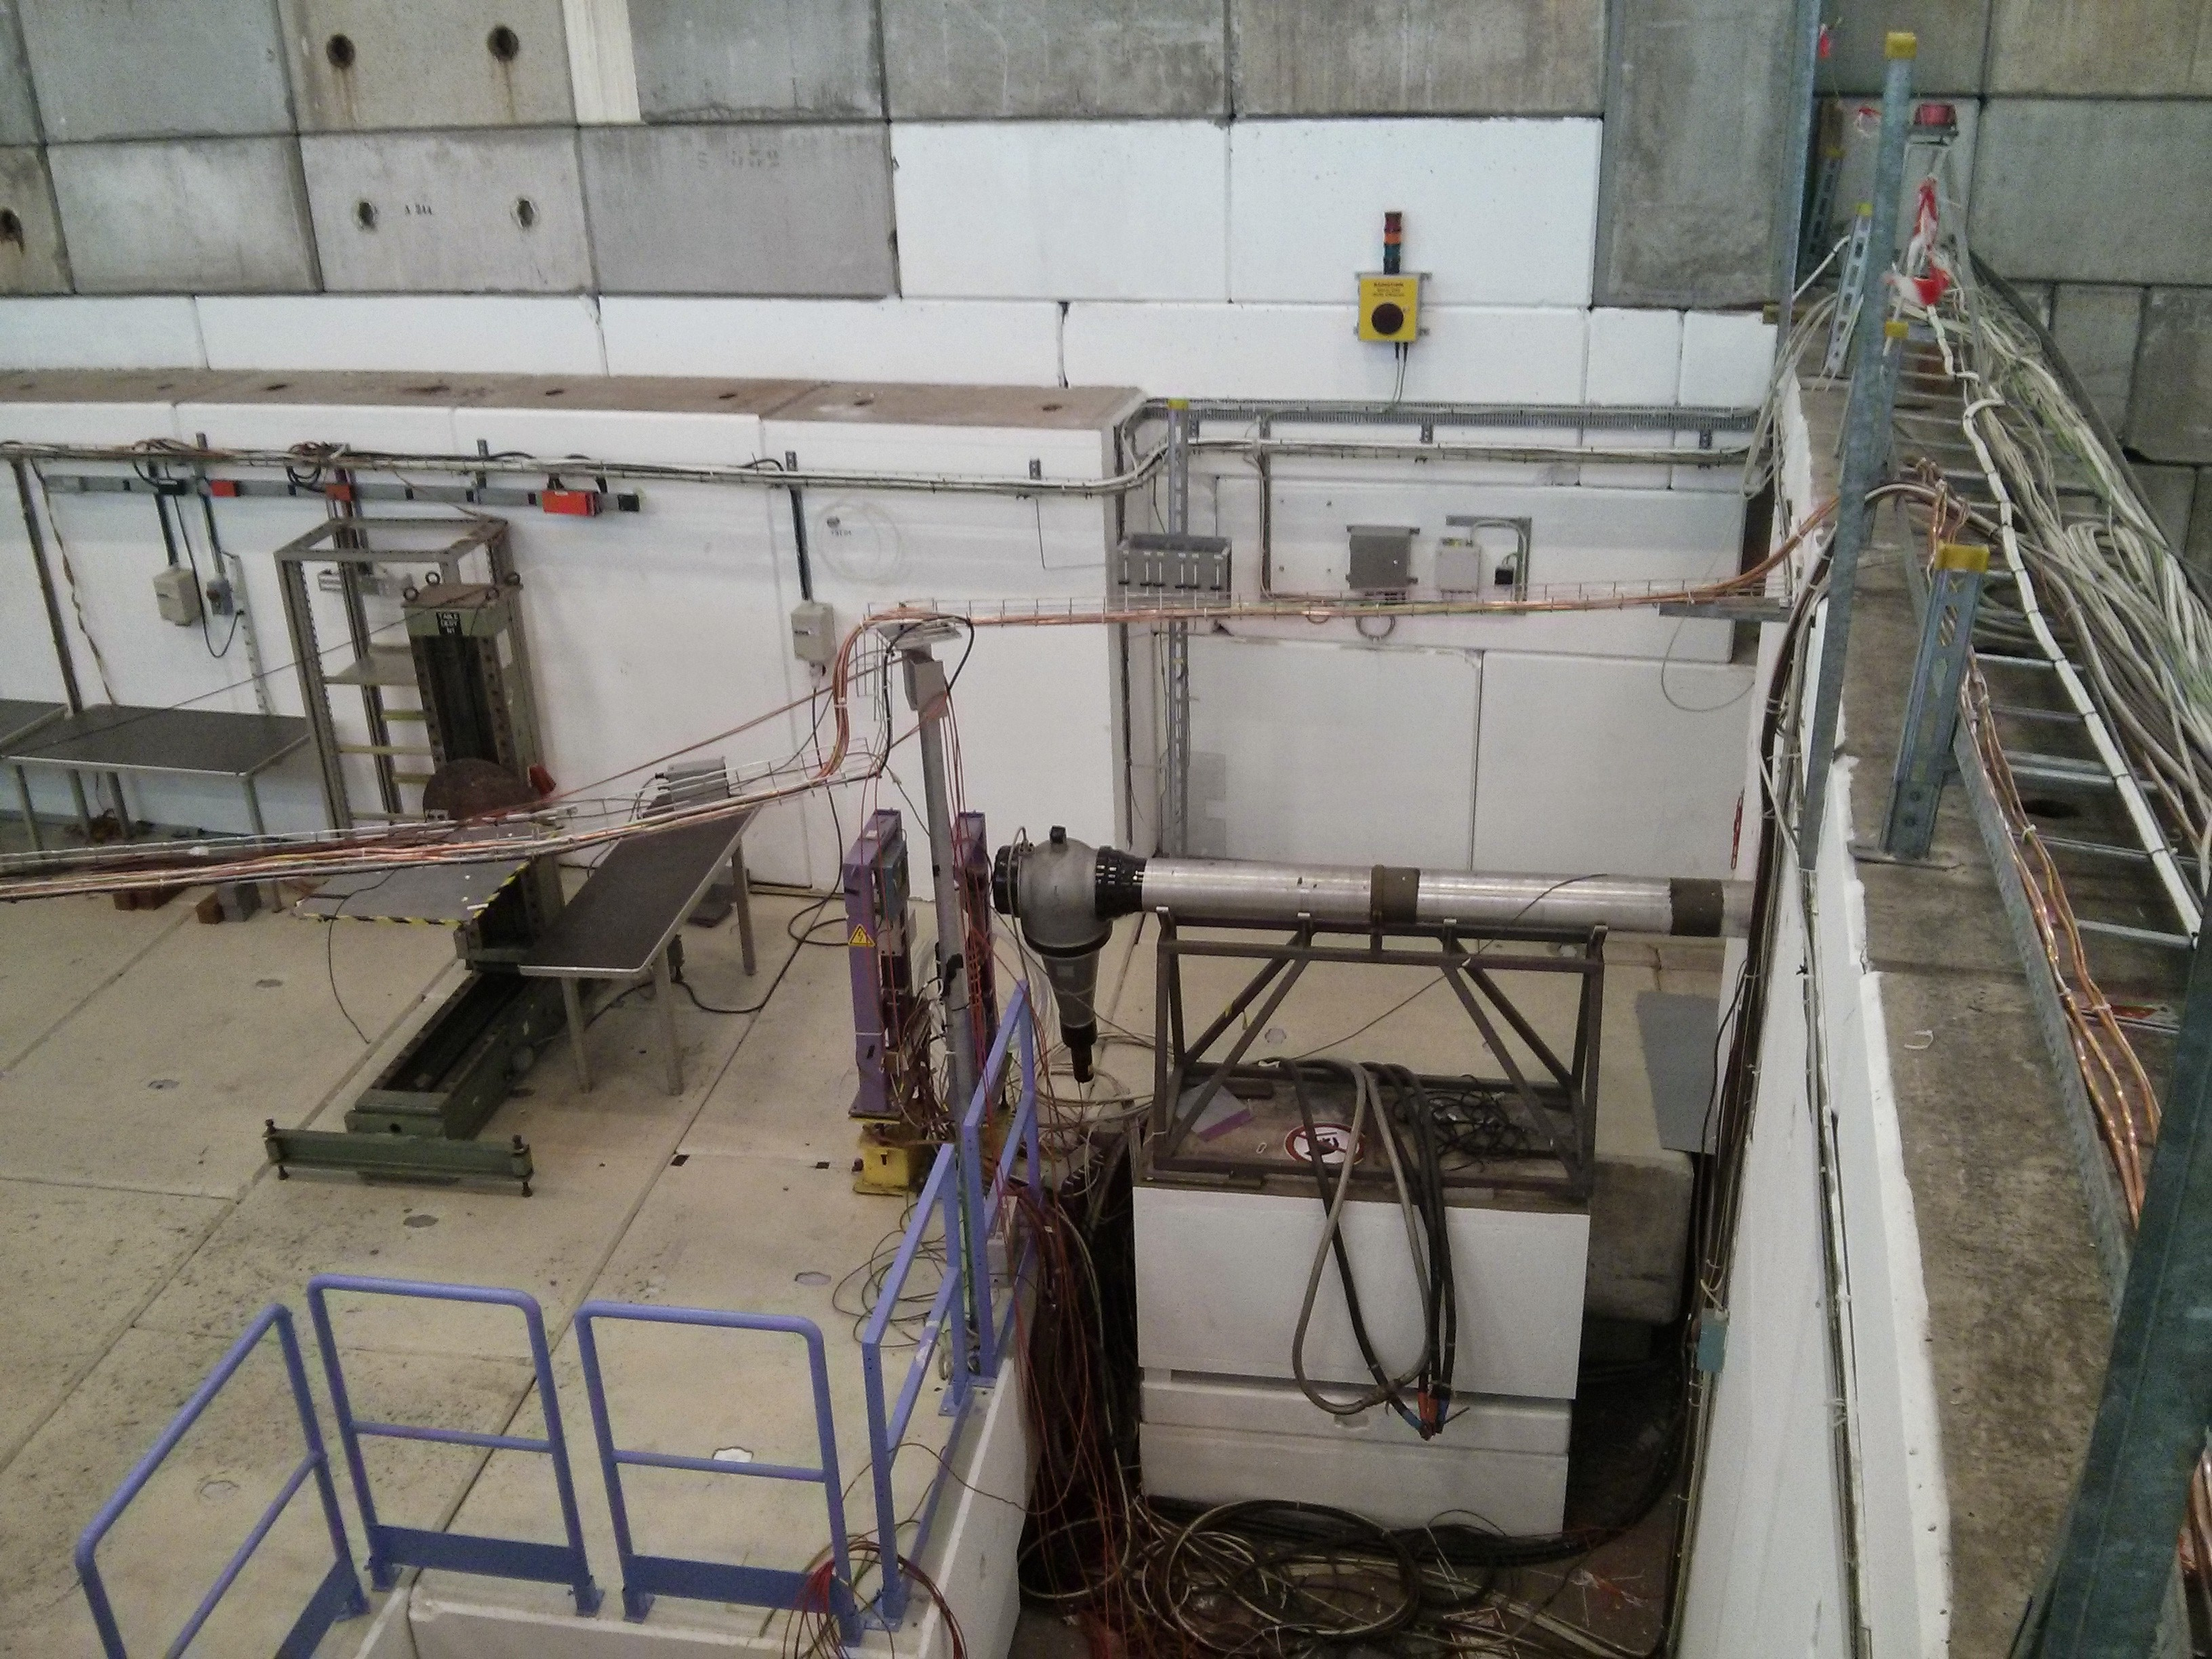
\includegraphics[scale=0.075]{img/beamline.jpg}
  \end{figure}
\end{frame}

\begin{frame}{Components}
\begin{itemize}
\item{Cherenkov counters}
\item{Scintillators}
\item{Drift Wire Chambers}
\item{\color{red}Timepix}
\item{\color{red}MRPC}
\item{Lead-Glass Calorimeter (from Opal!)}
\item{\color{red}Straw Tracker (from Zeus!)}
\end{itemize}
Also, absorbers for electrons/muons and a 0.96T magnet.
\end{frame}

\section{MRPC}
\begin{frame}{Multigap RPC}
New detector for the 2015 competition.

High efficiency tracking detector with excellent time resolution ($\sim80\,\text{ps}$).

Technology used in the ALICE ToF detector - NINO Front-End cards.
\end{frame}

\begin{frame}{Anode PCB}
  \begin{figure}
    \centering
    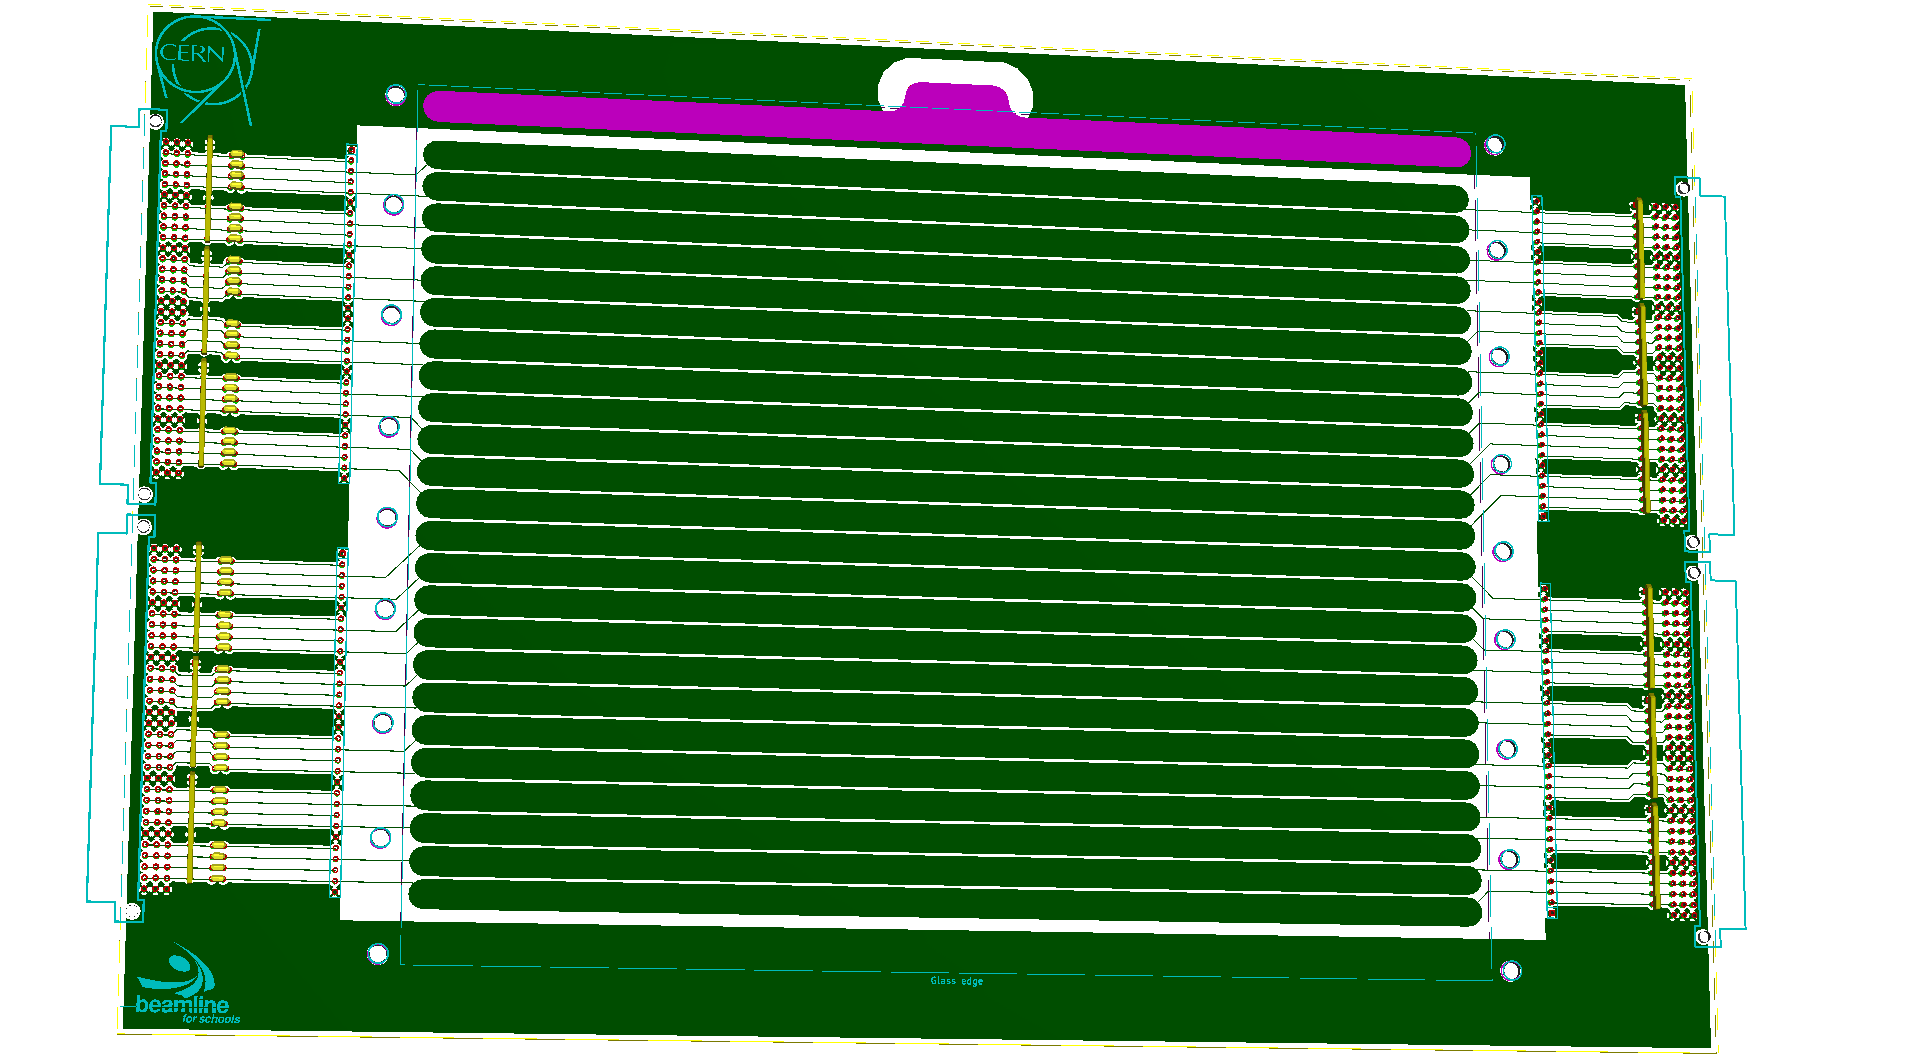
\includegraphics[scale=0.14]{img/anode-topside_white.png}
  \end{figure}
\end{frame}

\begin{frame}{Anode PCB}
  \begin{figure}
    \centering
    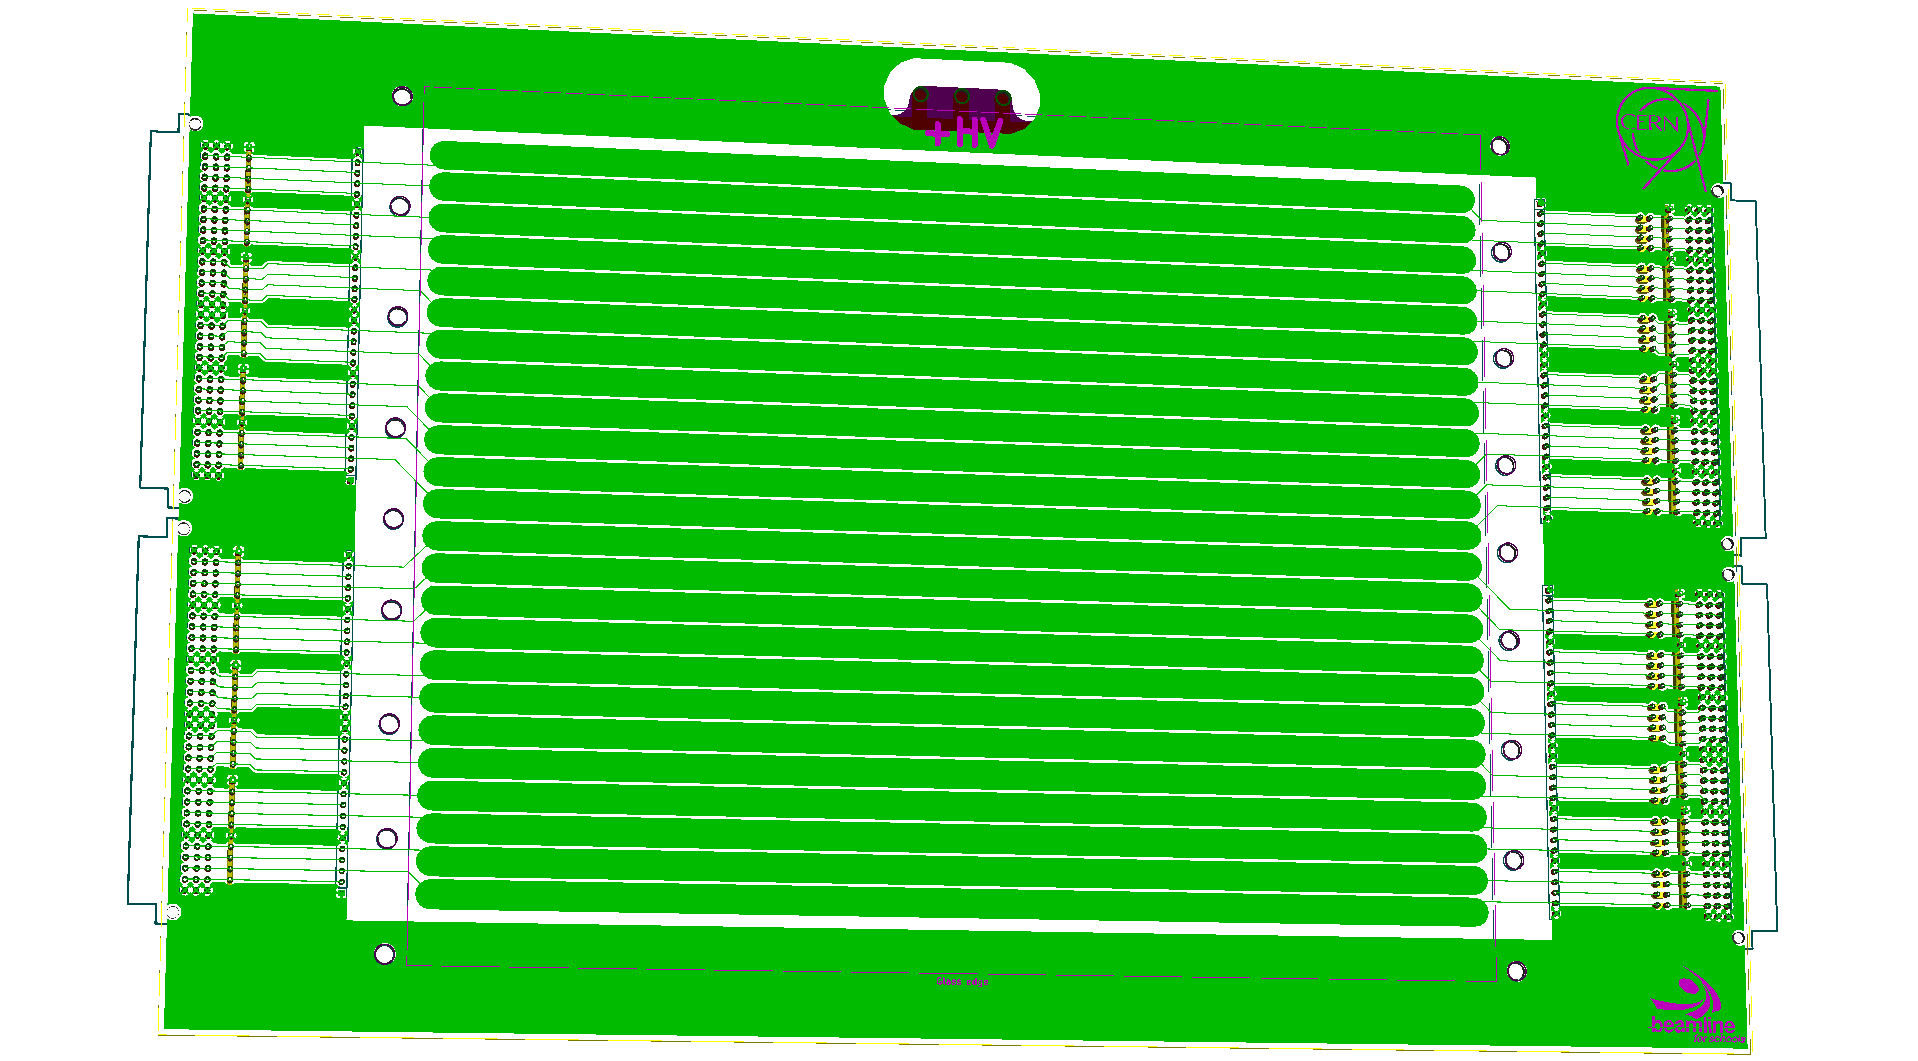
\includegraphics[scale=0.14]{img/anode-underside_white.png}
  \end{figure}
\end{frame}

\begin{frame}{Cathode PCB}
  \begin{figure}
    \centering
    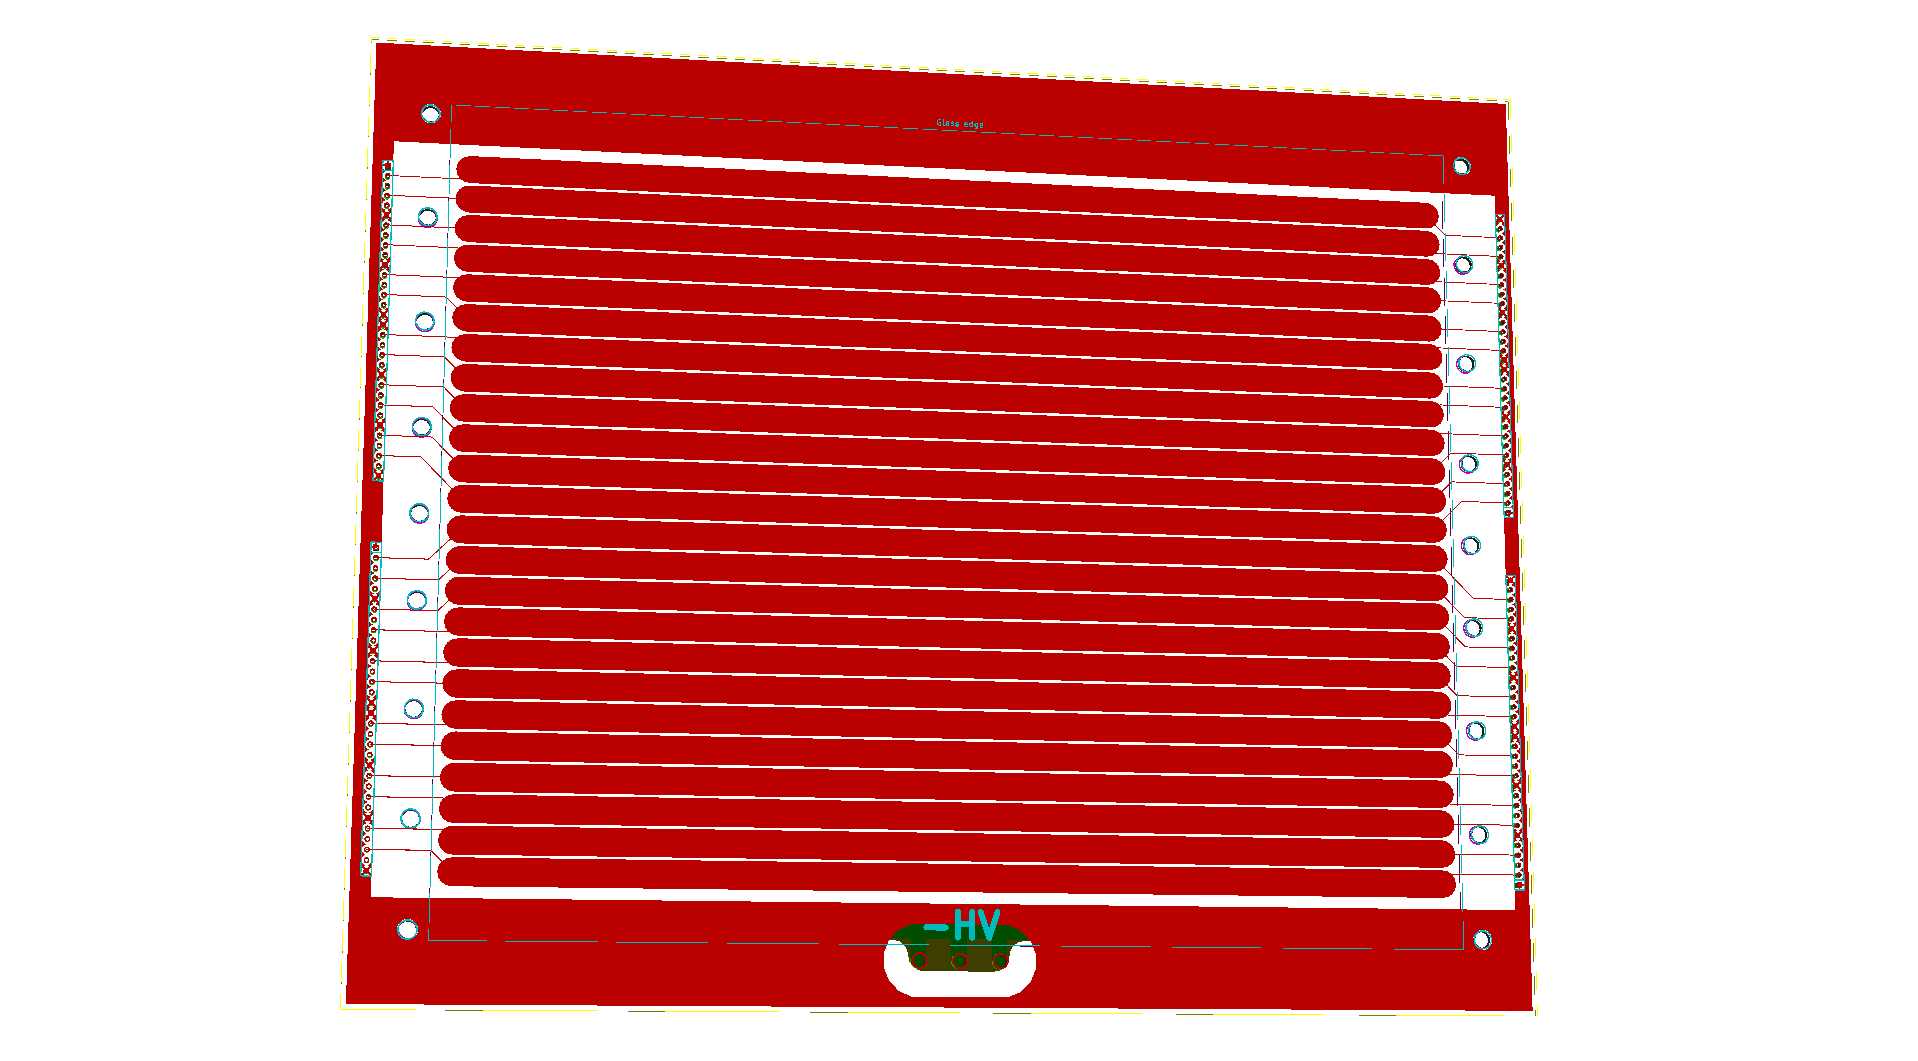
\includegraphics[scale=0.082]{img/cathode-topside_white.png}
    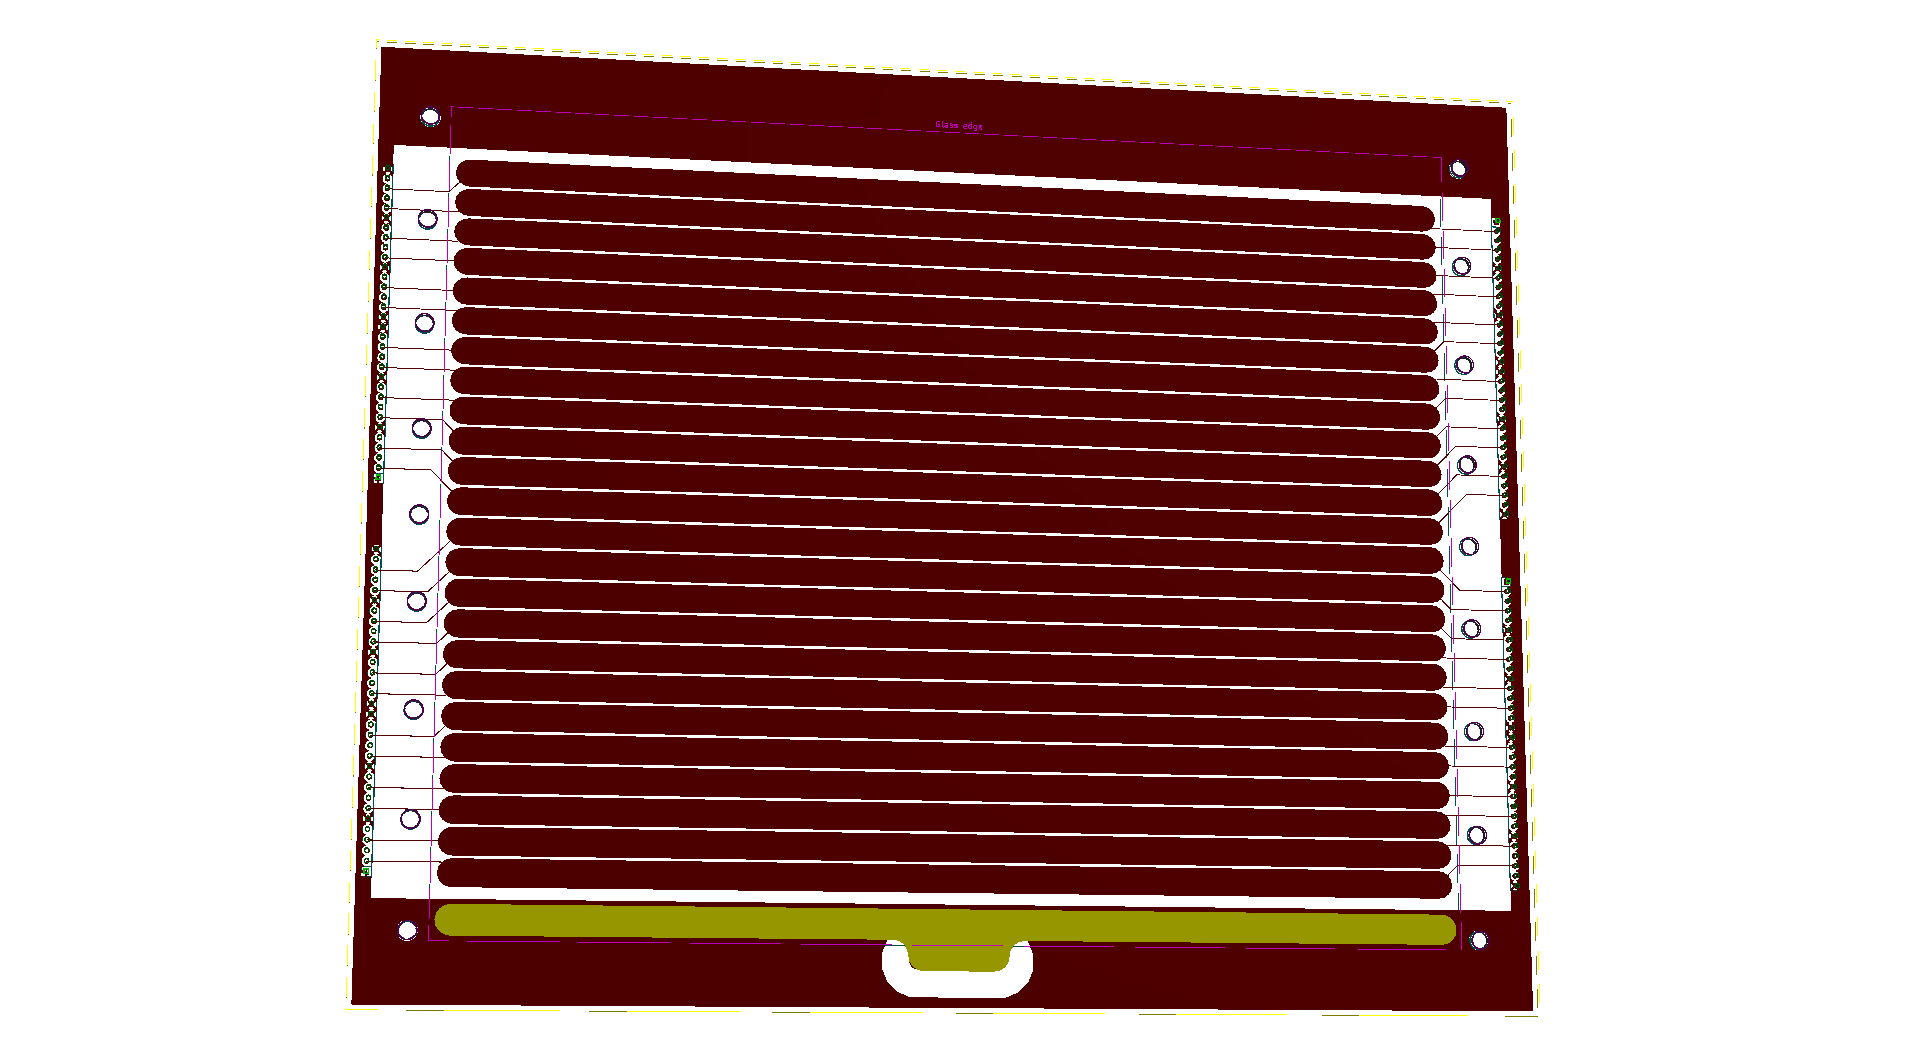
\includegraphics[scale=0.082]{img/cathode-underside_white.png}
  \end{figure}
\end{frame}

\begin{frame}{NINO interface}
  \begin{figure}
    \centering
    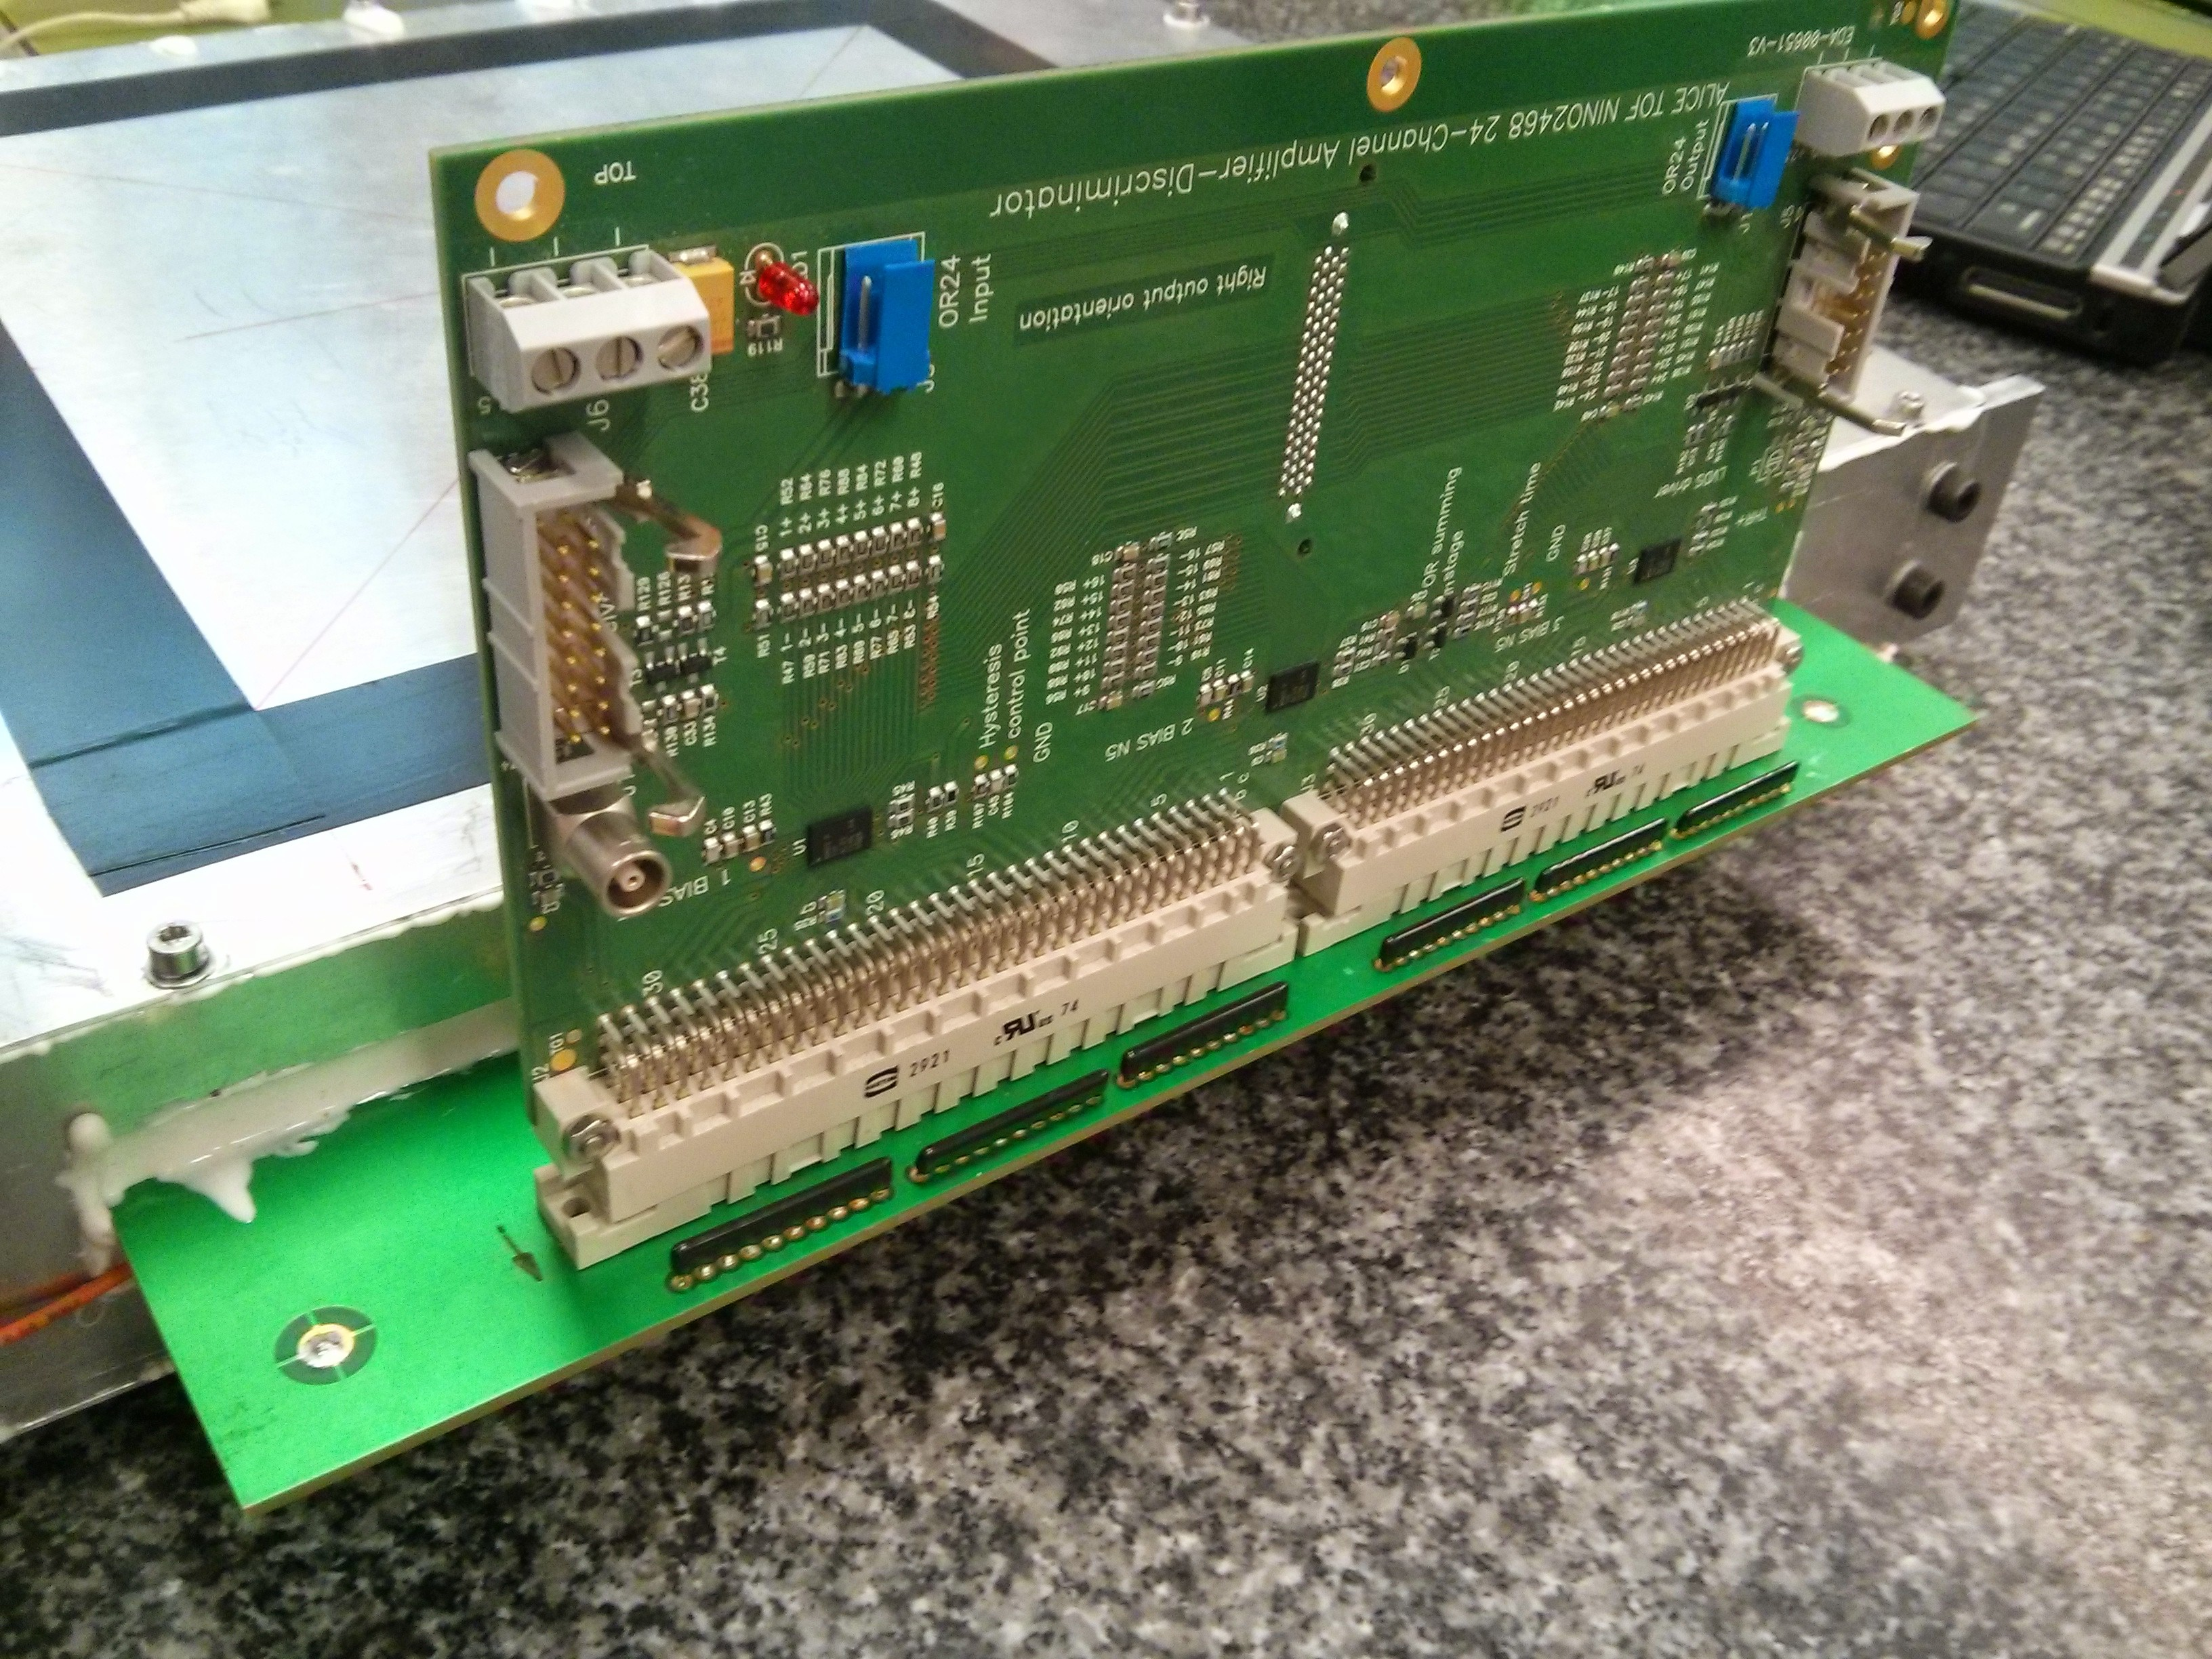
\includegraphics[scale=0.075]{img/NINO_card.jpg}
  \end{figure}
\end{frame}

\section[]{STT}
\begin{frame}{Straw Tracker}
  \begin{figure}
    \centering
    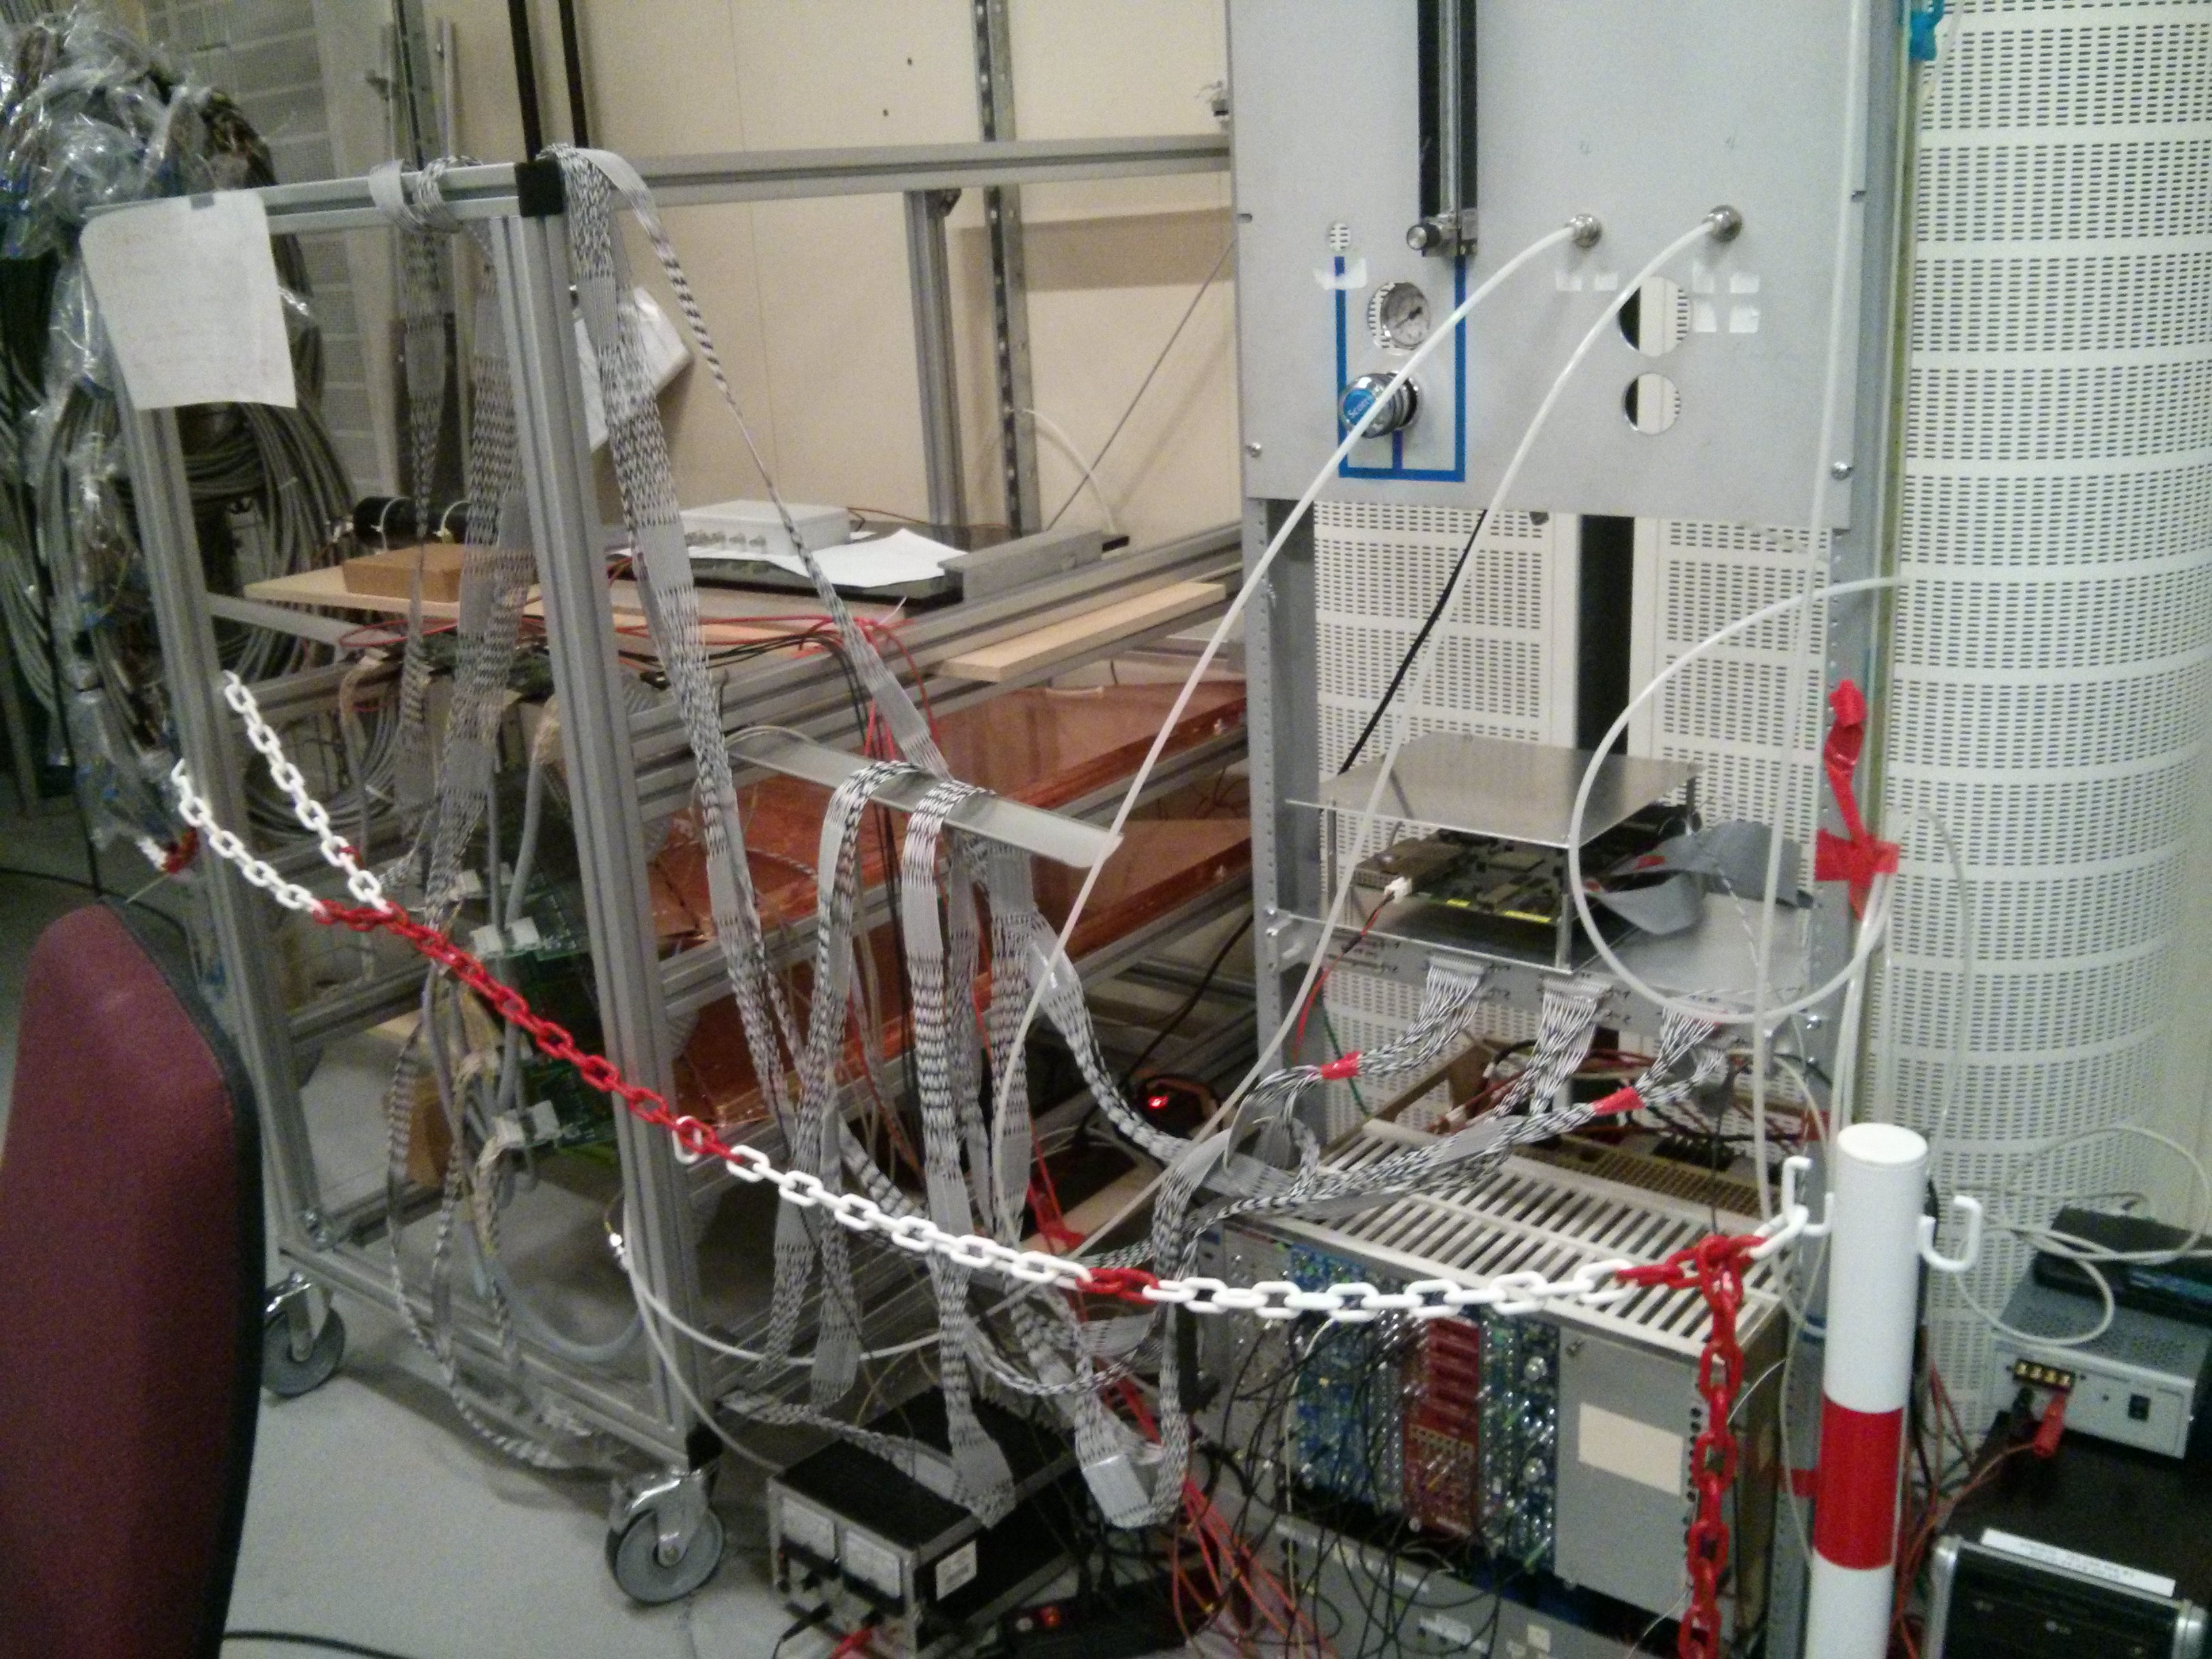
\includegraphics[scale=0.075]{img/STT.jpg}
  \end{figure}
\end{frame}

\section{ATLAS}
\begin{frame}{ATLAS work}
Joining an ATLAS test beam study in a few weeks, investigating Krypton gas in the TRT straws.

Trained for ROS on-call, need to book shifts.

Trained for Run Control, need to find time for shadow shifts.

\centering{\color{red} THESIS \& VIVA}
\end{frame}

\end{document}
